\documentclass{strrespaper-journ}
\usepackage[utf8]{inputenc}
\usepackage{csquotes}
\usepackage[english]{babel}

% For better tables
\usepackage{booktabs}
\usepackage[flushleft]{threeparttable}

% For images
\usepackage{graphicx}

% Required for the citations
\usepackage[style=apa,sortcites=true,sorting=nyt,backend=biber]{biblatex}
\addbibresource{../sample/bibliographies/str.bib} % Add your BibLaTeX files here

\title{Title of the Project: Should not Exceed 250 Characters}

\addAuthor{Ana Victoria R. Lloren} % Student 1
\addAuthor{Mc Jervis S. Villaruel} % Student 2
\addAuthor{Donna Salve C. Hipolito} % Student 3

\addAuthor{Rose Mary B. Butaran} % Research Adviser
\addAuthor{Ana Maria A. Chupungco} % Research Teacher

\affiliation{Philippine Science High School --- Main Campus, Department of Science and Technology, Agham Road, Diliman, \\Quezon City, 1101, Philippines}

\email{author@pshs.edu.ph}

\abstract{Abstract should BE written in \underline{one paragraph not to exceed 300 words}. It should summarize the background and scope of the work, the principal results, and note the implications of these results or main conclusions. it should concisely capture the basic content of the paper and be understandable without the text. References and acronyms should be avoided.}
\keywords{up to six; key; words; reflecting; content; paper} % Should be arranged alphabetically and separated by semicolon (This example is not)

\begin{document}
    \maketitle

    \section{Introduction}
	    Journal paper should be written a maximum of 7 pages excluding references section.
	    On the bottom of the page, list up to six key words that reflect the content of the paper arranged alphabetically (Santos, 2016). % This is personal communication

	    An Introduction should describe the paper’s background and provide the rationale for the present study.
	    Cite only those references that will provide the most relevant background rather than an exhaustive review of the topic (Santos \& Reyes, 2017). % This is personal communication too

    \section{Methodology}
	    \subsection{Subheading for Procedure 1}
	        Methods should be described concisely and clearly to allow experiments to be repeated. For commonly used methods, a simple reference is sufficient. Avoid references that are not readily accessible.

    \section{Results}
	    \subsection{Subheading for Result 1}
	        In Results, present data in only one of the following: text, table, or figure. Results should preferably have no more than five illustrations (tables and/or figures). Do not use tables or figures to present data that can be more concisely stated in the text. Discussion should interpret results in relation to previously published work. Do not repeat results or reiterate the introduction.
	        \begin{table}[htbp]
	            \begin{threeparttable}
	                \caption{Table Label Should be Concise and in Title Case \tnote{a}}
	                \label{tab:concise_table}
	                \begin{tabular}{cccc}
	                    \toprule
	                    Criteria Number & A (units)       & B (units)       & C (units)       \\
	                    \midrule
	                    1               & 1 \(\pm \) 0.01 & 1 \(\pm \) 0.01 & 1 \(\pm \) 0.01 \\
	                    2               & 1 \(\pm \) 0.01 & 1 \(\pm \) 0.01 & 1 \(\pm \) 0.01 \\
	                    3               & 1 \(\pm \) 0.01 & 1 \(\pm \) 0.01 & 1 \(\pm \) 0.01 \\
	                    4               & 1 \(\pm \) 0.01 & 1 \(\pm \) 0.01 & 1 \(\pm \) 0.01 \\
	                    \bottomrule
	                \end{tabular}
	                \begin{tablenotes}
	                    \item[a] Note: Type each table on a separate sheet.
	                    Never use vertical lines to separate columns.
	                    Prepare tables so that compared data read down, not across.
	                    Columns that show no significant variations should be omitted.
	                    Do not use tables for word lists.
	                    Titles should be clear, and column headings should be brief with units of measurements in parenthesis.
	                    Symbols and abbreviations should be defined below the table.
	                    Indicate table footnotes with a, b, c, etc.
	                    Do not present the same data in both graphical and tabular form.
	                    Tables should be self-explanatory or understandable without reference to the text.
	                \end{tablenotes}
	            \end{threeparttable}
	        \end{table}

	        \begin{figure}[htbp]
	            \centering
	            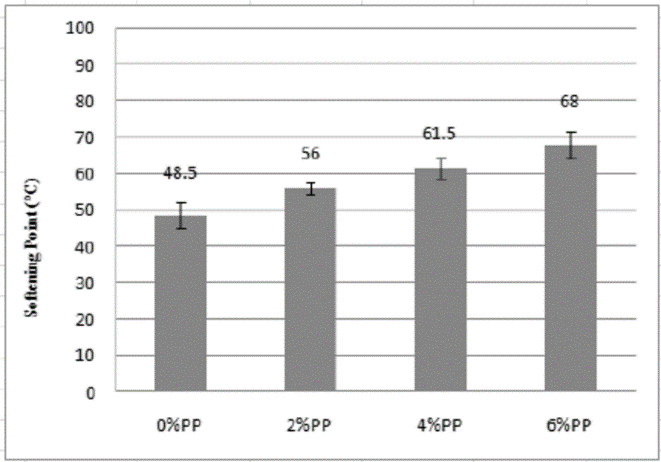
\includegraphics[width=\linewidth]{../sample/graphics/bar_graph}
	            \caption{Figure label should be in sentence case ending in period, placed under the figure.  Each figure should have a legend or caption and should be self-explanatory. Figure legends should be in lowercase print-type, except for the first letter of first word. Abbreviations and symbols on figures should be defined in the legend. Figures include line drawings, photographs, and computer plots. They should be clear.}
	            \label{fig:bar_graph}
	        \end{figure}

    \section{Discussion}
	    Discussion should incorporate referencing of the figures or data tables presented in the Results section. Literature citations should be selective, not to exceed 30 references for a research paper.

    \section{Summary and Conclusion}
	    Point out significant findings of the study in relation to the objectives of the study. Include your recommendations in this section.

    \section{Acknowledgement}
	    Acknowledgments should be brief and are placed under a separate heading immediately before References. Acknowledge any financial support for the work being published and personal assistance.

	    \nocite{letcher_wind_2017}
	    \nocite{al-shemmeri_wind_2010}
	    \nocite{trewby_wind_2014}

    \printbibliography
    % The example bibliographical entries were in APA 6th so it is recommended that you simply generate a .bib file using software such as Zotero and use BibLaTeX to format the citations and bibliography for you.
\end{document}